\documentclass[aspectratio=169]{beamer}

\usetheme{metropolis}
\usepackage[utf8]{inputenc}
\usepackage{graphicx}
\usepackage{booktabs}
\usepackage{textpos}
\usepackage{tikz}
\usetikzlibrary{arrows.meta, positioning, fit}

\graphicspath{{../reports/figures/}}

\definecolor{flowerBlue}{HTML}{2A78D6}
\definecolor{flowerOrange}{HTML}{EB6834}
\definecolor{flowerAqua}{HTML}{1BAF7A}
\definecolor{flowerRed}{HTML}{E34948}

\setbeamercolor{palette primary}{bg=flowerBlue,fg=white}
\setbeamercolor{progress bar}{fg=flowerOrange,bg=flowerBlue!20}
\setbeamercolor{alerted text}{fg=flowerOrange}
\setbeamercolor{example text}{fg=flowerAqua}

\title{Flower Species Classification with Deep Learning}
\subtitle{Comparing a CNN Trained from Scratch to a Pretrained EfficientNetB0 on the Oxford Flowers 102 Dataset}
\author{Ana Nicuesa}
\date{\today}

\begin{document}

\maketitle

\begin{frame}{Evaluator's map: this talk $\leftrightarrow$ the repository}
\small
\begin{tabular}{p{2.9cm}p{4.6cm}p{3.3cm}}
\toprule
\textbf{Repo path} & \textbf{What's there} & \textbf{In this talk} \\
\midrule
\texttt{notebooks/01-05} & EDA, preprocessing, training, evaluation, summary & Acts II \& III \\
\texttt{src/data/} & Split, augmentation & Act II \\
\texttt{src/models/} & Baseline CNN, EfficientNetB0, training loop & Act II \\
\texttt{src/evaluation/} & Accuracy, calibration, thresholds & Act III \\
\texttt{tests/} & Unit tests for all of the above & throughout \\
\texttt{app/app.py} & Streamlit demo & Act III \\
\texttt{docs/} & Business case, model card, architecture & Act III \\
\bottomrule
\end{tabular}

\vspace{0.8em}
Every claim in this presentation can be traced back to the repository.
\end{frame}

% ================================================================
% ACT I --- THE CHALLENGE
% ================================================================
\section{Act I --- The Challenge}

\begin{frame}{Motivation: automated flower species identification}
Identifying a flower's exact species from a photograph requires domain
expertise that most people do not have, and manual identification using
field guides does not scale.

\vspace{1em}
\begin{itemize}
  \item Non-expert users, such as home gardeners, retail staff, or hikers,
    typically cannot distinguish visually similar species such as
    \emph{Canterbury bells} and \emph{sweet pea}.
  \item A trained botanist can make this distinction reliably. A computer
    vision model can potentially do the same, at a much larger scale.
\end{itemize}

\vspace{1em}
This motivates the central question addressed in this project: whether a
model can reach this level of accuracy in practice, not just in principle.
\end{frame}

\begin{frame}{Why this task is suitable for automation}
\begin{columns}[T]
  \column{0.5\textwidth}
  \textbf{Who would use this}
  \begin{itemize}
    \item Consumer plant-ID apps
    \item E-commerce / nursery catalogs
    \item Citizen-science biodiversity tools
    \item Botany education
  \end{itemize}

  \column{0.5\textwidth}
  \textbf{Why it's a good fit}
  \begin{itemize}
    \item Visual, repetitive, high-volume
    \item Low cost of an incorrect prediction
    \item Pretrained vision models already encode useful features
  \end{itemize}
\end{columns}

\vspace{1em}
A reliable classifier can convert an expert-dependent task into a
self-service solution, provided that low-confidence predictions are
identified rather than presented as certain.
\end{frame}

\begin{frame}{Why this is a hard computer vision problem}
This is not a coarse-grained classification problem such as distinguishing
cats from cars. It requires distinguishing 102 categories within a single
type of object, based on subtle differences in petal shape, color gradient,
and cluster pattern.

\vspace{1em}
\begin{itemize}
  \item Some species are visually near-identical
  \item Photos vary in lighting, angle, background, and framing
  \item Some species have substantially fewer example photos than others
\end{itemize}

\vspace{1em}
\emph{Fine-grained classification} — distinguishing closely related
categories rather than unrelated ones — is one of the most challenging
problems in computer vision.
\end{frame}

\begin{frame}{Why this is an interesting machine learning problem}
Given the limited and unevenly distributed data per category, there are two
standard approaches:

\vspace{1em}
\begin{enumerate}
  \item Train a model from randomly initialized weights, using only the
    data available for this task.
  \item Reuse a model already trained to extract visual features from a
    different, larger task, and adapt it to this one.
\end{enumerate}

\vspace{1em}
Transfer learning (option 2) is widely used in practice. In theory,
features learned from large natural-image datasets, such as edges,
textures, and shapes, should transfer well to flower images, since flowers
are also natural images. Rather than assuming transfer learning works,
this project evaluates that assumption experimentally.
\end{frame}

\begin{frame}{The research question}
\centering
\vspace{1em}
{\Large\itshape ``Can transfer learning outperform a CNN trained from
scratch on a fine-grained image classification problem?''}

\vspace{2em}
\normalsize\normalfont
This question is tested empirically. The remainder of this presentation is
organized around answering it.
\end{frame}

% ================================================================
% ACT II --- THE INVESTIGATION
% ================================================================
\section{Act II --- The Investigation}

\begin{frame}{Oxford Flowers 102}
\begin{columns}[T]
  \column{0.55\textwidth}
  \begin{itemize}
    \item 102 flower species
    \item 8{,}189 images total
    \item Custom stratified split: 6{,}551 train / 819 validation / 819 test
    \item Loaded via \texttt{tensorflow-datasets} — no manual downloads
  \end{itemize}

  \column{0.45\textwidth}
  \includegraphics[width=\textwidth]{01_sample_images.png}
\end{columns}

\vspace{0.05em}
{\scriptsize\color{black!55}\textrightarrow\ \texttt{src/data/dataset.py}, \texttt{notebooks/01\_data\_exploration.ipynb}}
\end{frame}

\begin{frame}{Class imbalance is hidden by the official split}
\begin{center}
\includegraphics[width=0.75\textwidth]{01_class_distribution.png}
\end{center}
\small The official split allocates exactly 10 training images to every
class. This is a controlled but artificial design. When all 8{,}189 images
are pooled together, the class distribution is uneven: some species have up
to 258 images, others as few as 40. This project uses a stratified
80/10/10 re-split of the pooled data so that this class imbalance can be
analyzed directly, rather than being hidden by the benchmark's original
split.

\vspace{0.05em}
{\scriptsize\color{black!55}\textrightarrow\ \texttt{src/data/dataset.py:load\_raw\_combined}, \texttt{tests/test\_data.py}}
\end{frame}

\begin{frame}{Image resolution and format}
\begin{center}
\includegraphics[width=0.85\textwidth]{01_resolution_histograms.png}
\end{center}
\small All images are RGB, \texttt{uint8}, with no exceptions. Raw
resolutions are mostly between 500 and 700 pixels, with a maximum of
1{,}168 pixels. Resizing to a fixed $224\times224$ input is therefore
always a downscaling operation.

\vspace{0.05em}
{\scriptsize\color{black!55}\textrightarrow\ \texttt{notebooks/01\_data\_exploration.ipynb}, section ``Image Characteristics''}
\end{frame}

\begin{frame}{Aspect ratio and geometric distortion}
\begin{columns}[T]
  \column{0.55\textwidth}
  \includegraphics[width=\textwidth]{01_aspect_ratio_distribution.png}

  \column{0.45\textwidth}
  \small Aspect ratio ranges from 0.43 (portrait) to 2.05 (landscape).
  Resizing every image to a square does not crop the content; it introduces
  geometric distortion for the approximately 9\% of images at the extremes
  of this range. This trade-off is acknowledged rather than hidden.
  \vspace{0.5em}

  \textbf{Dataset passed every integrity check}: no invalid dimensions, no
  unexpected channel counts, no NaNs.
\end{columns}
\end{frame}

\begin{frame}{Examples: size and aspect-ratio extremes}
\begin{center}
\includegraphics[width=0.7\textwidth]{01_image_characteristic_examples.png}
\end{center}
\end{frame}

\begin{frame}{Experimental design: two training approaches}
Both approaches are trained on the same data, and the results are compared
directly, rather than assuming in advance which one performs better:

\vspace{1em}
\begin{columns}[T]
  \column{0.5\textwidth}
  \textbf{Path A --- trained from scratch}\\
  A small neural network, trained to recognize flowers using only the
  6{,}551 training photos. No prior visual knowledge.

  \column{0.5\textwidth}
  \textbf{Path B --- transfer learning}\\
  A model already trained to extract visual features from a much larger,
  unrelated task, adapted to the 102 flower species in this dataset.
\end{columns}

\vspace{1em}
\emph{The next two slides describe each approach. All other variables are
then controlled so that the comparison is informative.}
\end{frame}

\begin{frame}{Path A: a small CNN trained from scratch}
\footnotesize
A \textbf{CNN} (convolutional neural network) processes an image through a
sequence of stages, referred to here as \textbf{blocks}. Each block detects
patterns and passes a reduced representation to the next block, so that
increasingly complex features are extracted at deeper stages:

\vspace{0.3em}
\begin{center}
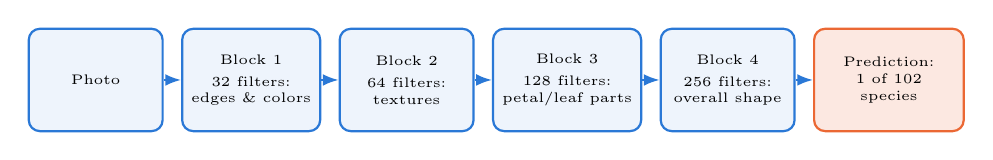
\begin{tikzpicture}[
  box/.style={draw=flowerBlue, thick, rounded corners, fill=flowerBlue!8,
    minimum height=1.3cm, minimum width=1.7cm, align=center, font=\tiny},
  outbox/.style={draw=flowerOrange, thick, rounded corners, fill=flowerOrange!15,
    minimum height=1.3cm, minimum width=1.9cm, align=center, font=\tiny},
  arr/.style={-{Latex[length=2mm]}, thick, flowerBlue}
]
\node[box] (img) {Photo};
\node[box, right=0.22cm of img] (b1) {Block 1\\[2pt]32 filters:\\edges \& colors};
\node[box, right=0.22cm of b1] (b2) {Block 2\\[2pt]64 filters:\\textures};
\node[box, right=0.22cm of b2] (b3) {Block 3\\[2pt]128 filters:\\petal/leaf parts};
\node[box, right=0.22cm of b3] (b4) {Block 4\\[2pt]256 filters:\\overall shape};
\node[outbox, right=0.22cm of b4] (out) {Prediction:\\1 of 102\\species};
\draw[arr] (img) -- (b1);
\draw[arr] (b1) -- (b2);
\draw[arr] (b2) -- (b3);
\draw[arr] (b3) -- (b4);
\draw[arr] (b4) -- (out);
\end{tikzpicture}
\end{center}

\vspace{0.2em}
A \textbf{filter} is the basic pattern detector: a small sliding window that
responds to one specific shape or color pattern. A \textbf{block} groups
many filters into a single stage. The number of filters increases from 32
to 256 across the four blocks, so deeper blocks represent more complex
features.

\vspace{0.2em}
The term \textbf{``small, 4-block''} refers to a compact architecture with
only four stages. This model has no prior visual knowledge: all parameters
are learned exclusively from the training images in this project.

\vspace{0.05em}
{\scriptsize\color{black!55}\textrightarrow\ \texttt{src/models/build\_model.py:build\_baseline\_cnn}}
\end{frame}

\begin{frame}{Path B: transfer learning with EfficientNetB0}
\footnotesize
Path B reuses a network already trained on a much larger, unrelated task,
instead of training from randomly initialized weights:

\vspace{0.4em}
\begin{center}
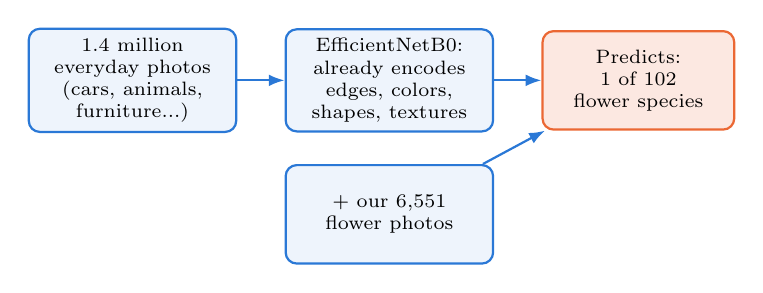
\begin{tikzpicture}[
  box/.style={draw=flowerBlue, thick, rounded corners, fill=flowerBlue!8,
    minimum height=1.25cm, text width=2.4cm, align=center, font=\scriptsize},
  outbox/.style={draw=flowerOrange, thick, rounded corners, fill=flowerOrange!15,
    minimum height=1.25cm, text width=2.2cm, align=center, font=\scriptsize},
  arr/.style={-{Latex[length=2mm]}, thick, flowerBlue}
]
\node[box] (data1) {1.4 million everyday photos\\(cars, animals, furniture...)};
\node[box, right=0.6cm of data1] (model) {EfficientNetB0:\\already encodes edges, colors, shapes, textures};
\node[outbox, right=0.6cm of model] (out) {Predicts:\\1 of 102 flower species};
\node[box, below=0.4cm of model, text width=2.4cm] (data2) {+ our 6{,}551 flower photos};
\draw[arr] (data1) -- (model);
\draw[arr] (model) -- (out);
\draw[arr] (data2) -- (out);
\end{tikzpicture}
\end{center}

\vspace{0.2em}
\textbf{EfficientNetB0} (Google, 2019) is the name of this pretrained
model. It was selected for its accuracy-to-size trade-off rather than for
being the largest available model. Only the final classification step,
distinguishing flower species, is learned in this project; the general
visual features (edges, colors, shapes) are inherited from pretraining at
no additional training cost.

\vspace{0.05em}
{\scriptsize\color{black!55}\textrightarrow\ \texttt{src/models/build\_model.py:build\_transfer\_model}}
\end{frame}

\begin{frame}{Data augmentation strategy}
\begin{columns}[T]
  \column{0.5\textwidth}
  \textbf{Augmentation}\\
  Mild random horizontal flip, rotation, zoom, and contrast adjustment,
  implemented as model layers. It is therefore active automatically during
  training and inactive during evaluation.
  \includegraphics[width=\textwidth]{02_augmentation_examples.png}

  \column{0.5\textwidth}
  \textbf{Why mild augmentation}\\
  Flower species are partly distinguished by color and shape. Strong
  augmentation would remove the visual cues needed to separate similar
  species, so only mild transformations are applied.
\end{columns}

\vspace{0.05em}
{\scriptsize\color{black!55}\textrightarrow\ \texttt{src/data/augmentation.py}}
\end{frame}

\begin{frame}{Two-stage transfer learning}
\begin{enumerate}
  \item \textbf{Frozen backbone.} Only the newly added classification head
    is trained. The pretrained EfficientNetB0 weights remain unchanged
    while the head learns to use the existing features.
  \item \textbf{Fine-tuning.} The top 20 backbone layers are unfrozen and
    trained with a learning rate 100 times lower than in the first stage,
    adapting the pretrained features to this dataset without substantially
    overwriting them.
\end{enumerate}

\vspace{1em}
\texttt{EarlyStopping}, \texttt{ModelCheckpoint}, and
\texttt{ReduceLROnPlateau} keep every run reproducible and stop each stage
at its best epoch automatically.

\vspace{0.05em}
{\scriptsize\color{black!55}\textrightarrow\ \texttt{src/models/train.py}, \texttt{notebooks/03\_model\_training.ipynb}}
\end{frame}

\begin{frame}{Validation of the data split}
\small
A valid comparison requires the test set to be index-disjoint from
training and validation, and unused during training or model selection.
This was verified directly:
\begin{itemize}
  \item The split is stratified and \textbf{reproducible}: identical on
    rerun with the same seed
  \item Train/validation/test index sets are provably \textbf{disjoint},
    with no overlap, by construction
  \item Every class keeps its natural share of images in every split — no
    class is dropped or over- or under-represented relative to the full
    dataset
\end{itemize}

\vspace{0.05em}
{\scriptsize\color{black!55}\textrightarrow\ \texttt{src/data/dataset.py:\_stratified\_split\_assignment}, \texttt{tests/test\_data.py}}
\end{frame}

\begin{frame}{A consistent comparison under the same data protocol}
\centering
\vspace{0.5em}
\begin{tabular}{ll}
\toprule
\textbf{Held constant} & \textbf{Varies} \\
\midrule
Same 6{,}551 training images & \\
Same preprocessing (resize, no rescale) & \\
Same augmentation & \textbf{Only the model:} \\
Same evaluation protocol \& test set & from scratch, or pretrained? \\
Same random seed & \\
\bottomrule
\end{tabular}

\vspace{1.5em}
\normalsize Both approaches use the same train, validation and test split,
the same input resolution, the same augmentation strategy and the same
evaluation protocol. The architectures and their optimization strategies
necessarily differ. This design makes the performance difference
informative while acknowledging that the two architectures require
different training strategies.
\end{frame}

% ================================================================
% ACT III --- THE DISCOVERY
% ================================================================
\section{Act III --- The Discovery}

\begin{frame}{Path A: the from-scratch CNN reaches a clear performance ceiling}
\begin{center}
\includegraphics[width=0.85\textwidth]{03_baseline_training_curves.png}
\end{center}
The baseline learns progressively, but validation performance is noisy and
plateaus far below the transfer-learning model. Learning useful
fine-grained features from scratch is difficult with this amount of data.
\end{frame}

\begin{frame}{Path B: training and validation accuracy improve together}
\begin{center}
\includegraphics[width=0.85\textwidth]{03_transfer_frozen_training_curves.png}
\end{center}
Training and validation accuracy increase together throughout training.
This indicates that the pretrained ImageNet features already provide most
of the relevant representational capacity.
\end{frame}

\begin{frame}{Test-set accuracy comparison}
\begin{center}
\includegraphics[width=0.46\textwidth]{04_test_accuracy_comparison.png}
\end{center}
\begin{center}
\Large\alert{60.0\%} $\rightarrow$ \Large\textbf{95.8\%}\\[2pt]
\normalsize on 819 held-out test images the models never saw during training.
\end{center}

{\scriptsize\color{black!55}\textrightarrow\ \texttt{notebooks/04\_evaluation.ipynb}}
\end{frame}

\begin{frame}{Why transfer learning outperforms the baseline}
\small
\begin{itemize}
  \item EfficientNetB0 was pretrained on \textbf{1.4 million images} before
    being applied to this task, and already encodes general visual
    features such as edges, textures, colors, and shapes.
  \item The CNN trained from scratch has to learn equivalent low-level
    features in addition to the 102-class distinction, using only
    6{,}551 training images.
  \item Given the limited amount of training data relative to the
    difficulty of the task, this pretraining advantage accounts for most
    of the performance difference observed.
\end{itemize}

\vspace{1em}
\normalsize This directly answers the research question: transfer learning
outperforms training from scratch by \alert{35.8 percentage points} under
this experimental setup.
\end{frame}

\begin{frame}{Effect of fine-tuning}
Fine-tuning produces a modest but consistent improvement on both validation
and test performance:

\begin{center}
\begin{tabular}{lccc}
\toprule
Model & Test accuracy & Macro F1 \\
\midrule
Transfer (frozen) & 94.4\% & 93.6\% \\
Transfer (fine-tuned) & \textbf{95.8\%} & \textbf{95.2\%} \\
\bottomrule
\end{tabular}
\end{center}

\vspace{1em}
Unfreezing a small part of the backbone at a low learning rate improves
adaptation to the flower dataset without substantially disrupting the
pretrained representation.
\end{frame}

\begin{frame}{Error analysis: confused class pairs}
\begin{center}
\includegraphics[width=0.62\textwidth]{04_most_confused_pairs.png}
\end{center}
\small Classification errors are concentrated on specific pairs of visually
similar species, rather than distributed randomly across all classes.
\end{frame}

\begin{frame}{Per-class F1 score variation}
\begin{center}
\includegraphics[width=0.5\textwidth]{04_per_class_f1_extremes.png}
\end{center}
\small Macro-averaged F1, which weights every class equally, reveals this
variation. Overall accuracy does not.
\end{frame}

\begin{frame}{Examples of confident correct predictions}
\begin{center}
\includegraphics[width=\textwidth]{04_sample_predictions_correct.png}
\end{center}
\end{frame}

\begin{frame}{Examples of confident incorrect predictions}
\begin{center}
\includegraphics[width=\textwidth]{04_sample_predictions_incorrect.png}
\end{center}
The model's most confident errors are almost always visually similar
species, rather than arbitrary misclassifications.
\end{frame}

\begin{frame}{Top-k accuracy}
\small With 102 visually similar species, top-1 accuracy is a strict
metric: a correct species ranked second still counts as an error.
Reporting the top-$k$ candidates provides additional information:

\vspace{0.8em}
\begin{center}
\begin{tabular}{lccc}
\toprule
& Top-1 & Top-3 & Top-5 \\
\midrule
Accuracy & 95.8\% & \textbf{99.0\%} & 99.3\% \\
\bottomrule
\end{tabular}
\end{center}

\vspace{0.8em}
Most top-1 errors correspond to the correct species being ranked second or
third, rather than an unrelated prediction.
\end{frame}

\begin{frame}{Model calibration}
\begin{columns}[T]
  \column{0.5\textwidth}
  \includegraphics[width=\textwidth]{04_reliability_diagram.png}

  \column{0.5\textwidth}
  \small A well-calibrated model's predicted confidence should match its
  empirical accuracy, shown as the dashed line. This model's Expected
  Calibration Error is \textbf{0.020}.

  \vspace{0.5em}
  Confidence also separates correct from incorrect predictions: mean
  confidence is \textbf{95.4\%} when correct and \textbf{63.7\%} when
  incorrect. These results support a prototype abstention rule, although
  further validation would be required before deployment.
\end{columns}

{\scriptsize\color{black!55}\textrightarrow\ \texttt{src/evaluation/metrics.py:expected\_calibration\_error}}
\end{frame}

\begin{frame}{Confidence threshold for abstention}
\begin{center}
\includegraphics[width=0.42\textwidth]{04_risk_coverage_curve.png}
\end{center}
\small A confidence threshold trades \emph{coverage} (the proportion of
predictions accepted automatically) for accuracy on the accepted
predictions. The threshold (\textbf{0.7}) was selected using validation
data only (92.1\% coverage, 98.9\% accuracy) and then evaluated once on the
held-out test set (91.9\% coverage, 98.5\% accuracy). Selecting the
threshold on the same data used for final evaluation would invalidate the
results.

{\scriptsize\color{black!55}\textrightarrow\ \texttt{src/evaluation/metrics.py:coverage\_selective\_accuracy}}
\end{frame}

\begin{frame}{Demonstration application}
A lightweight Streamlit application wraps the fine-tuned model. Users
upload a photo and receive the top-5 predicted species with associated
confidence values.

\vspace{0.5em}
\begin{center}

\includegraphics[width=0.85\textwidth]{00_app_screenshot.png}
\end{center}

\begin{itemize}
  \item Low-confidence predictions are flagged rather than presented as fact
  \item Same 224$\times$224 preprocessing pipeline as training — no
    train/inference mismatch
  \item Run locally with \texttt{streamlit run app/app.py}
\end{itemize}

\vspace{0.05em}
{\scriptsize\color{black!55}\textrightarrow\ \texttt{app/app.py}}
\end{frame}

\begin{frame}{Requirements for production deployment}
\begin{itemize}
  \item \textbf{Out-of-distribution handling} — a confidence threshold or
    dedicated detector for species outside the training set
  \item \textbf{Broader, noisier training data} — real user photos are
    less controlled than this benchmark
  \item \textbf{Monitoring} — track confidence drift over time, collect
    corrections
  \item \textbf{Latency/footprint validation} for the target platform
    (mobile vs. server)
  \item \textbf{Licensing check} on training data and deployed weights
\end{itemize}

\vspace{0.05em}
{\scriptsize\color{black!55}\textrightarrow\ \texttt{docs/business\_case.md}, \texttt{docs/model\_card.md}}
\end{frame}

\begin{frame}{Final lessons learned}
\footnotesize
\textbf{Summary:} transfer learning outperforms training from scratch in
this experiment. This result follows from a controlled comparison, not
from an assumption made in advance.

\vspace{0.4em}
\textbf{What I would apply in future projects:}
\begin{itemize}
  \setlength{\itemsep}{1pt}
  \item \emph{Verify the experimental setup before interpreting results.}
    The official data split concealed the class imbalance that this
    project needed to analyze; identifying this issue changed the overall
    approach.
  \item \emph{Be precise about methodology.} ``Fair'' and ``controlled''
    comparisons only make sense if you clearly explain what stayed
    constant and what changed.
  \item \emph{Accuracy alone is not sufficient.} Calibration and
    confidence estimates are needed to apply a research result in a
    practical system.
  \item \emph{A held-out test set must be verified, not assumed.} Checking
    that the confidence threshold was selected using validation data, not
    test data, identified and corrected a methodological error.
\end{itemize}

{\scriptsize\color{black!55}\textrightarrow\ \texttt{notebooks/05\_project\_summary.ipynb}}
\end{frame}

\begin{frame}{Thank you}
\centering
\Large Questions?

\vspace{2em}
\normalsize
\textbf{GitHub Repository}\\[4pt]
\texttt{github.com/AnaNicuesa/Flowers}\\[4pt]
{\small Full code, notebooks, and reports}
\end{frame}

\end{document}
